\section{实验结果}
可执行代码见源码,使用方法见源码中的README,源码可从github上查看下载,地址https://github.com/zhang-x-z/CompilerPrincipal-Lab


测试选取了解析JSON格式的文件,并自己推到了DFA和LR1 Table,词法包括string,\{,\},number,[,],:,逗号,true,null,false以及空格(包括制表符换行),输入的dfa文件如下
\begin{lstlisting}
I0,0,{,I1,},I2,comma,I3,:,I4,[,I5,],I6,space,I7,cr,I7,lf,I7,tab,I7,t,I8,f,I9,n,I10,",I21,1,I24,2,I24,3,I24,4,I24,5,I24,6,I24,7,I24,8,I24,9,I24,-,I25,0,I26
I1,1
I2,1
I3,1
I4,1
I5,1
I6,1
I7,1
I8,0,r,I11
I9,0,a,I12
I10,0,u,I13
I11,0,u,I14
I12,0,l,I15
I13,0,l,I16
I14,0,e,I17
I15,0,s,I18
I16,0,l,I19
I17,1
I18,0,e,I20
I19,1
I20,1
I21,0,^"\,I21,\,I22,",I23
I22,0,",I21,\,I21,/,I21,b,I21,f,I21,n,I21,r,I21,t,I21
I23,1
I24,1,0,I24,1,I24,2,I24,3,I24,4,I24,5,I24,6,I24,7,I24,8,I24,9,I24,.,I27
I25,0,1,I24,2,I24,3,I24,4,I24,5,I24,6,I24,7,I24,8,I24,9,I24,0,I26
I26,1,.,I27
I27,0,0,I28,1,I28,2,I28,3,I28,4,I28,5,I28,6,I28,7,I28,8,I28,9,I28
I28,1,0,I28,1,I28,2,I28,3,I28,4,I28,5,I28,6,I28,7,I28,8,I28,9,I28
\end{lstlisting}
lexer配置文件如下
\begin{lstlisting}
dfa.location=./simple-json-dfa.csv
dfa.startName=I0
dfa.encoding=utf8
sourcecode.encoding=utf8
sourcecode.buffersize=50
sourcecode.location=./example.json
dfa.I1=left-brace
dfa.I2=right-brace
dfa.I3=comma
dfa.I4=colon
dfa.I5=left-bracket
dfa.I6=right-bracket
dfa.I7=whitespace
dfa.I17=true
dfa.I19=false
dfa.I20=null
dfa.I23=string
dfa.I24=number
dfa.I26=number
dfa.I28=number
\end{lstlisting}
输入的语法文件如下
\begin{lstlisting}
<?xml version="1.0" encoding="UTF-8" ?>
<grammar>
    <expression id="acc">
        <leftPart>
            S
        </leftPart>
        <rightPart>
            [object]
        </rightPart>
    </expression>
    <expression id="1">
        <leftPart>
            object
        </leftPart>
        <rightPart>
            [left-brace][right-brace]
        </rightPart>
    </expression>
    <expression id="2">
        <leftPart>
            object
        </leftPart>
        <rightPart>
            [left-brace][objects][right-brace]
        </rightPart>
    </expression>
    <expression id="3">
        <leftPart>
            objects
        </leftPart>
        <rightPart>
            [string][colon][value][comma][objects]
        </rightPart>
    </expression>
    <expression id="4">
        <leftPart>
            objects
        </leftPart>
        <rightPart>
            [string][colon][value]
        </rightPart>
    </expression>
    <expression id="5">
        <leftPart>
            value
        </leftPart>
        <rightPart>
            [string]
        </rightPart>
    </expression>
    <expression id="6">
        <leftPart>
            value
        </leftPart>
        <rightPart>
            [number]
        </rightPart>
    </expression>
    <expression id="7">
        <leftPart>
            value
        </leftPart>
        <rightPart>
            [object]
        </rightPart>
    </expression>
    <expression id="8">
        <leftPart>
            value
        </leftPart>
        <rightPart>
            [array]
        </rightPart>
    </expression>
    <expression id="9">
        <leftPart>
            value
        </leftPart>
        <rightPart>
            [true]
        </rightPart>
    </expression>
    <expression id="10">
        <leftPart>
            value
        </leftPart>
        <rightPart>
            [false]
        </rightPart>
    </expression>
    <expression id="11">
        <leftPart>
            value
        </leftPart>
        <rightPart>
            [null]
        </rightPart>
    </expression>
    <expression id="12">
        <leftPart>
            array
        </leftPart>
        <rightPart>
            [left-bracket][right-bracket]
        </rightPart>
    </expression>
    <expression id="13">
        <leftPart>
            array
        </leftPart>
        <rightPart>
            [left-bracket][values][right-bracket]
        </rightPart>
    </expression>
    <expression id="14">
        <leftPart>
            values
        </leftPart>
        <rightPart>
            [value][comma][values]
        </rightPart>
    </expression>
    <expression id="15">
        <leftPart>
            values
        </leftPart>
        <rightPart>
            [value]
        </rightPart>
    </expression>
</grammar>
\end{lstlisting}
输入的LR Table文件如下:\\
1.LR Action Table
\begin{lstlisting}
I0,left-brace,I2,0
I1,$,acc,2
I2,right-brace,I3,0,string,I4,0
I3,$,1,1
I4,colon,I6,0
I5,right-brace,I43,0
I6,string,I8,0,number,I9,0,true,I10,0,false,I11,0,null,I12,0,left-bracket,I15,0,left-brace,I16,0
I7,right-brace,4,1,comma,I17,0
I8,right-brace,5,1,comma,5,1
I9,right-brace,6,1,comma,6,1
I10,right-brace,9,1,comma,9,1
I11,right-brace,10,1,comma,10,1
I12,right-brace,11,1,comma,11,1
I13,right-brace,8,1,comma,8,1
I14,right-brace,7,1,comma,7,1
I15,right-bracket,I19,0,left-bracket,I20,0,left-brace,I30,0,string,I23,0,number,I24,0,true,I25,0,false,I26,0,null,I27,0
I16,right-brace,I31,0,string,I4,0
I17,string,I4,0
I18,right-brace,3,1
I19,right-brace,12,1,comma,12,1
I20,right-bracket,I33,0,string,I23,0,number,I24,0,true,I25,0,false,I26,0,null,I27,0
I21,right-bracket,I35,0
I22,right-bracket,15,1,comma,I36,0
I23,right-bracket,5,1,comma,5,1
I24,right-bracket,6,1,comma,6,1
I25,right-bracket,9,1,comma,9,1
I26,right-bracket,10,1,comma,10,1
I27,right-bracket,11,1,comma,11,1
I28,right-bracket,8,1,comma,8,1
I29,right-bracket,7,1,comma,7,1
I30,right-bracket,I37,0,string,I4,0
I31,right-bracket,1,1,comma,1,1
I32,right-bracket,I39,0
I33,right-bracket,12,1,comma,12,1
I34,right-bracket,I40,0
I35,right-brace,13,1,comma,13,1
I36,left-bracket,I20,0,left-brace,I30,0,string,I23,0,number,I24,0,true,I25,0,false,I26,0,null,I27,0
I37,right-bracket,1,1,comma,1,1
I38,right-brace,I44,0
I39,right-brace,2,1,comma,2,1
I40,right-bracket,13,1,comma,13,1
I41,right-bracket,14,1
I42,right-bracket,15,1,comma,I36,0
I43,$,2,1
I44,right-bracket,2,1,comma,2,1
\end{lstlisting}
2.LR Goto Table
\begin{lstlisting}
I0,object,I1
I2,objects,I5
I6,value,I7,array,I13,object,I14
I15,values,I21,value,I22,array,I28,object,I29
I16,objects,I32
I17,objects,I18
I20,values,I34,value,I22,array,I28,object,I29
I30,objects,I38
I36,values,I41,value,I42,array,I28,object,I29
\end{lstlisting}
parser配置文件
\begin{lstlisting}
lrTable.start=I0
lrActionTable.location=./json-actions.csv
lrGotoTable.location=./json-goto.csv
grammar.location=./json-grammar.xml
ignoreWhiteSpace=true
whiteSpace.name=whitespace
fileEncoding=UTF8
\end{lstlisting}
最后输出结果只是对语法分析树进行了层序遍历(顺序颠倒,输出的顺序是从右往左读每层语法分析树的结果),如图:\\
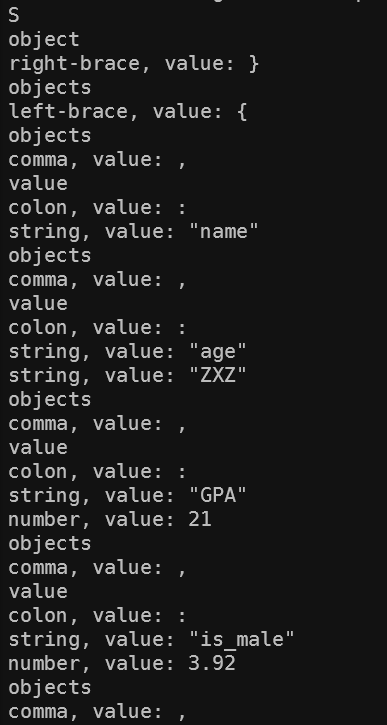
\includegraphics[scale=0.8]{1.png}\\
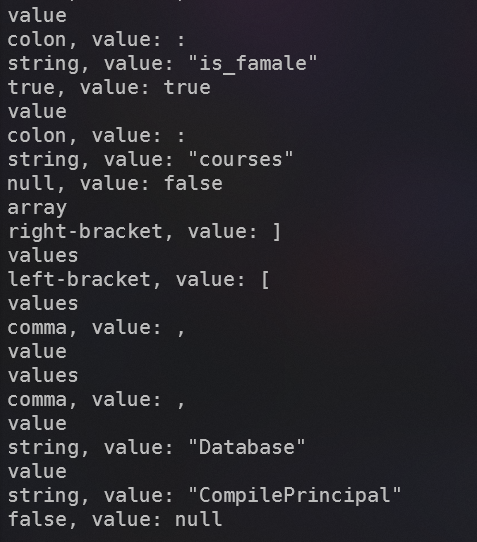
\includegraphics[scale=0.8]{2.png}